\section{Results}
Using the method proposed in scientific article \cite{1512356} allows to obtain the values in the table (\ref{tab:recapvalue}); it is observed that the distance between the robot’s actual parameters and the estimates are introduced by the assumed model simplifications and errors.
In the first analysis, the odometric center is placed in mid’s robot axle as well as in the model used, but this method does not take into account that the camera’s position may be not aligned with the point previously analyzed.
Errors also depend on assumptions regarding the non-deformability of the wheels, the tire above keyed and misalignments.
The motion is achieved by considering a regular and uniform surface, ignoring bumps, obstacles, unevenness, etc. 
In this scientific article, as in other scientific works \cite{censi13joint}--\cite{Jung2016}--\cite{DBLP:journals/ijrr/ChongK99}, is recommanded to use predetermined paths, possibly in a straight line, with counterclockwise and clockwise rotations in order to minimize errors and to allow independent calibration of the parameters.
On the other hand, for the results obtained from optimization we must take into account that there are limitations of the use of a genetic algorithm compared to alternative optimization algorithms.
From the optimization operation we get the solution for each path visible in the table \ref{tab:GAresult}, you can see that the values are slightly different for each dataset.
\begin{table}[!h]
\centering
\begin{adjustbox}{max width=0.45\textwidth}
	\pgfplotstableset{
	% global config, for example in the preamble
	% these columns/<colname>/.style={<options>} things define a style
	% which applies to <colname> only.
    every head row/.style={before row=\hline,after row=\hline},
    every last row/.style={after row=\hline},
    display columns/0/.style={column name =$r_\textsc{r}$, column type=r,fixed,fixed zerofill,precision=3,set thousands separator={\,}},
    display columns/1/.style={column name =$r_\textsc{l}$, column type=r,fixed,fixed zerofill,precision=3,set thousands separator={\,}},
    %other style option 
    display columns/2/.style={column name =b, column type=r, fixed,fixed zerofill,precision=3,set thousands separator={\,}},
    display columns/3/.style={column name =$\xi$, column type=r, fixed,fixed zerofill,precision=3,set thousands separator={\,}},
    display columns/4/.style={column name =d, column type=r, fixed,fixed zerofill,precision=3,set thousands separator={\,}},
    display columns/5/.style={column name =$\alpha$, column type=r, fixed,fixed zerofill,precision=3,set thousands separator={\,}},  
    }
    \pgfplotstabletypeset[col sep=space]{result.txt}
\end{adjustbox}
\caption{GA result}
\label{tab:GAresult}
\end{table}
Repeated fitness function evaluation for complex problems is often the most prohibitive and limiting segment of artificial evolutionary algorithms. Finding the optimal solution to complex high-dimensional, multimodal problems often requires very expensive fitness function evaluations.
The ``better" solution is only in comparison to other solutions. As a result, the stop criterion is not clear in every problem.
In many problems, GAs may have a tendency to converge towards local optima or even arbitrary points rather than the global optimum of the problem. This means that it does not ``know how" to sacrifice short-term fitness to gain longer-term fitness. The likelihood of this occurring depends on the shape of the fitness landscape: certain problems may provide an easy ascent towards a global optimum, others may make it easier for the function to find the local optima. 
This problem may be alleviated by using a different fitness function, increasing the rate of mutation, or by using selection techniques that maintain a diverse population of solutions, although the ``\emph{No Free Lunch theorem}" proves that there is no general solution to this problem. 
A common technique to maintain diversity is to impose a ``niche penalty", wherein, any group of individuals of sufficient similarity (niche radius) have a penalty added, which will reduce the representation of that group in subsequent generations, permitting other (less similar) individuals to be maintained in the population. This trick, however, may not be effective, depending on the landscape of the problem. 
Another possible technique would be to simply replace part of the population with randomly generated individuals, when most of the population is too similar to each other. Diversity is important in genetic algorithms (and genetic programming) because crossing over a homogeneous population does not yield new solutions. 
In evolution strategies and evolutionary programming, diversity is not essential because of a greater reliance on mutation.\columnbreak
\begin{figure}[!h]
   {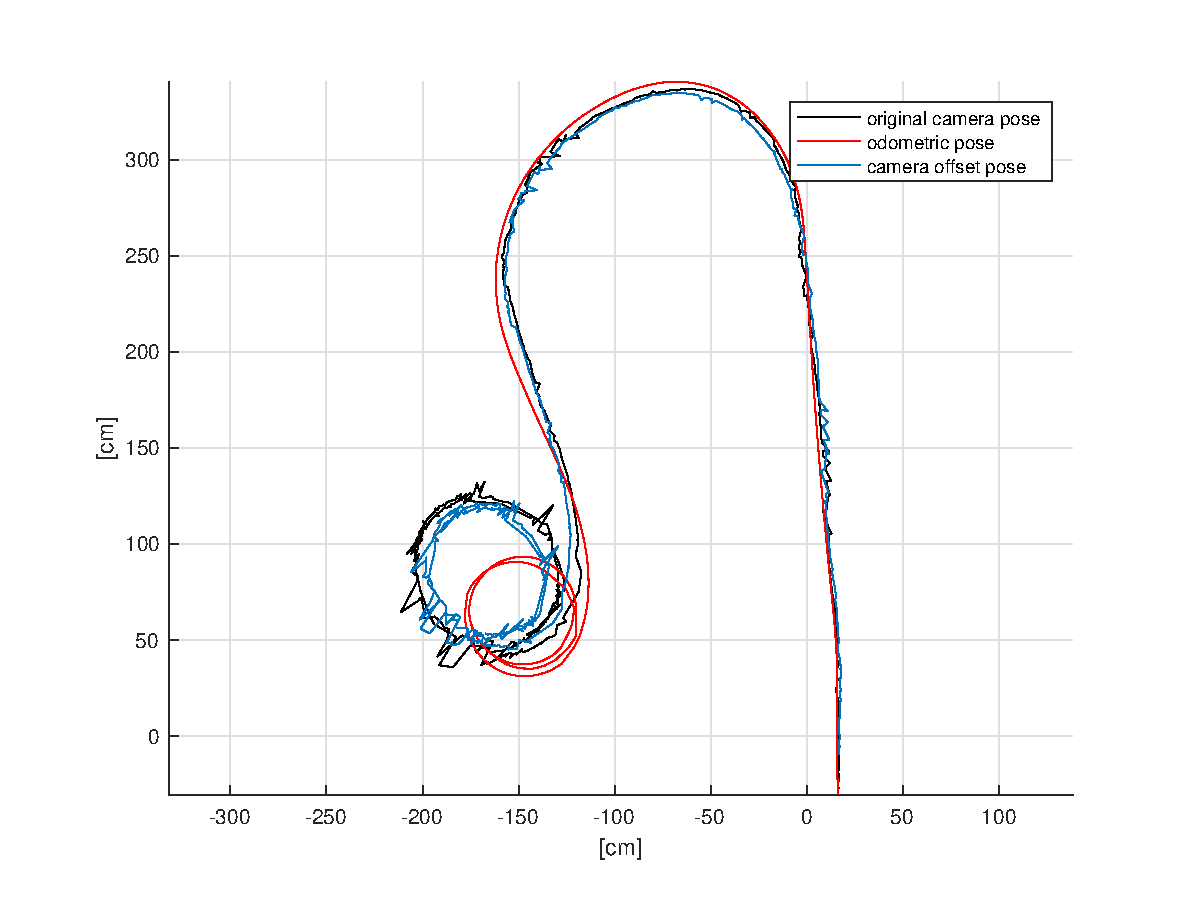
\includegraphics[width=0.45\textwidth]{recostropt_1}}\,
   \caption{Optimal odometric and camera position, dataset: 1}
   \label{fig:OptiOdo1}
\end{figure}
\begin{figure}[!h]
   {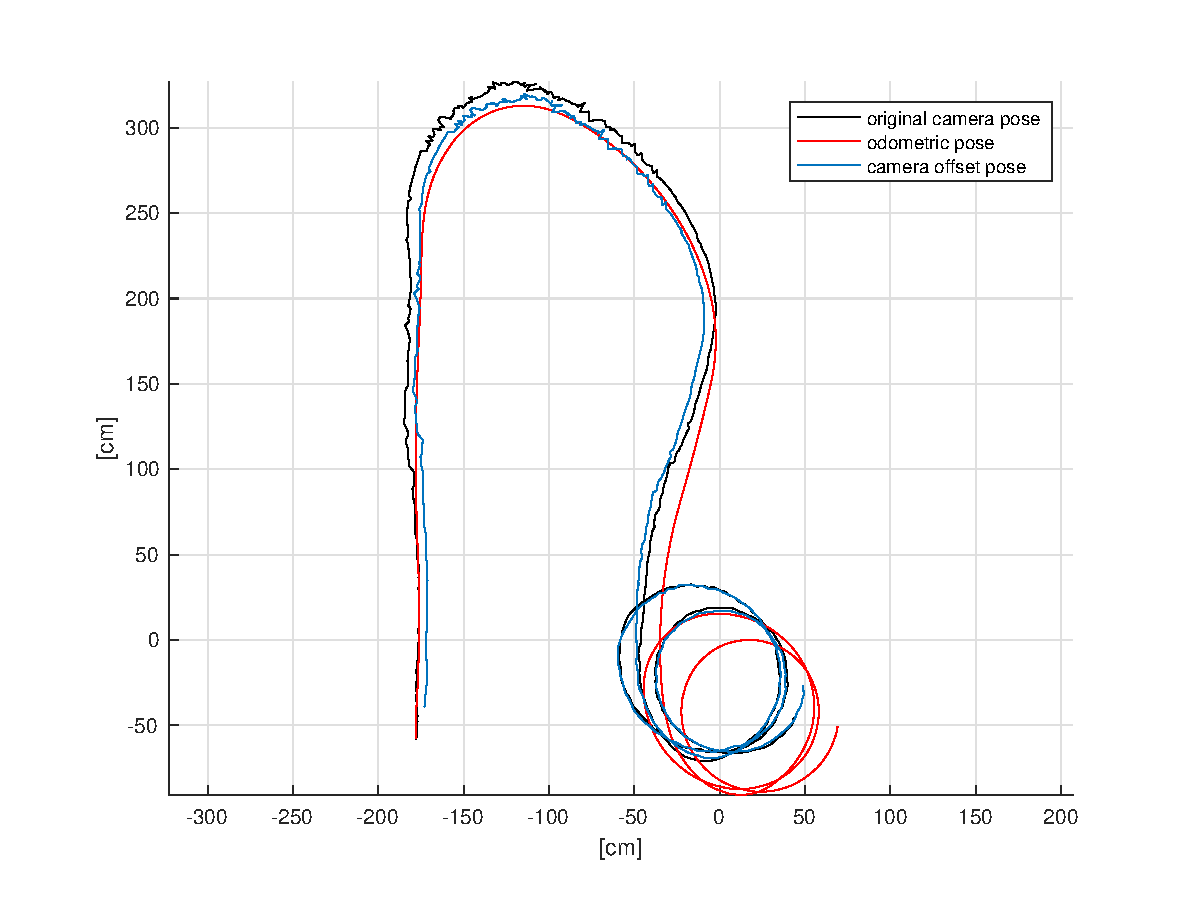
\includegraphics[width=0.45\textwidth]{recostropt_2}}\\
   \caption{Optimal odometric and camera position, dataset: 2}
   \label{fig:OptiOdo2}
\end{figure}
\begin{figure}[!htb]
   {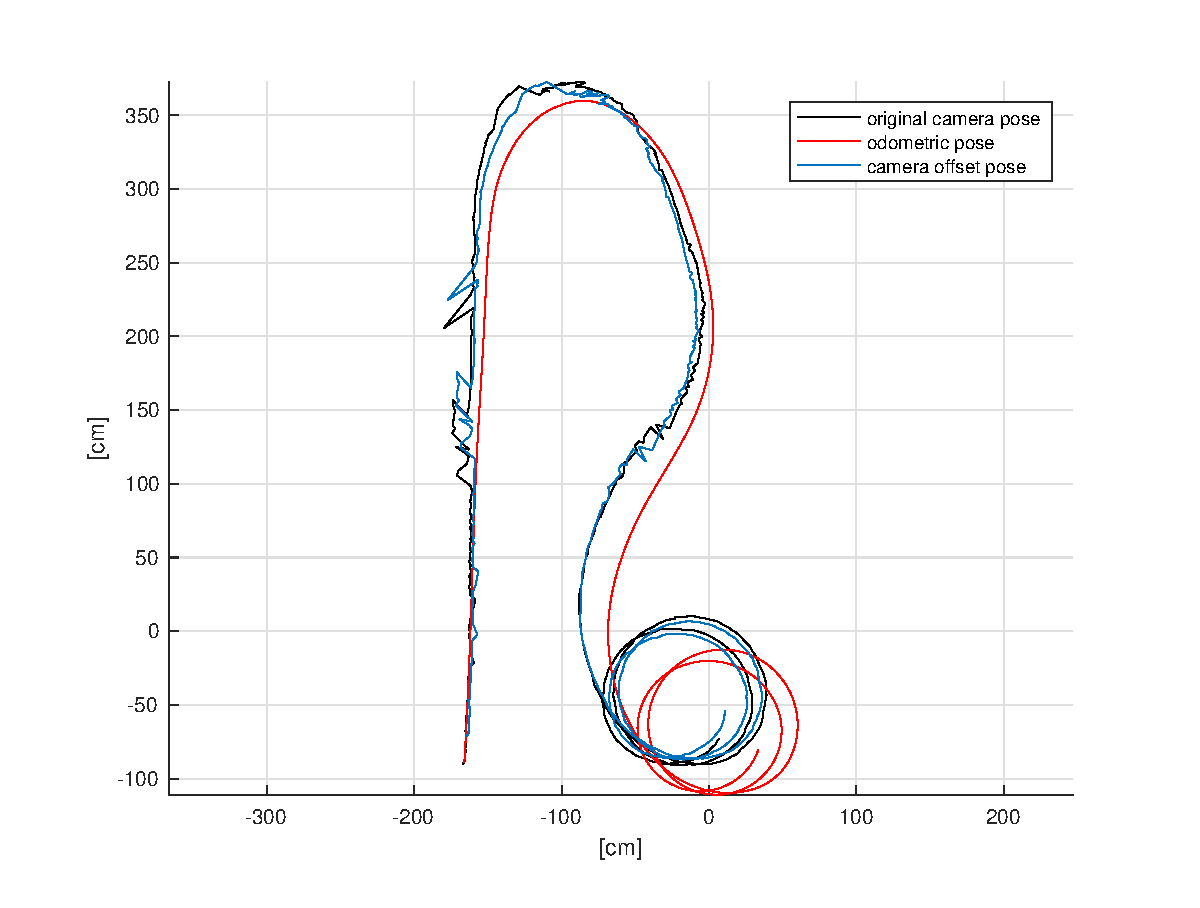
\includegraphics[width=0.45\textwidth]{recostropt_3}}\,
   \caption{Optimal odometric and camera position, dataset: 3}
   \label{fig:OptiOdo3}
\end{figure}
\begin{figure}[!htb]
   {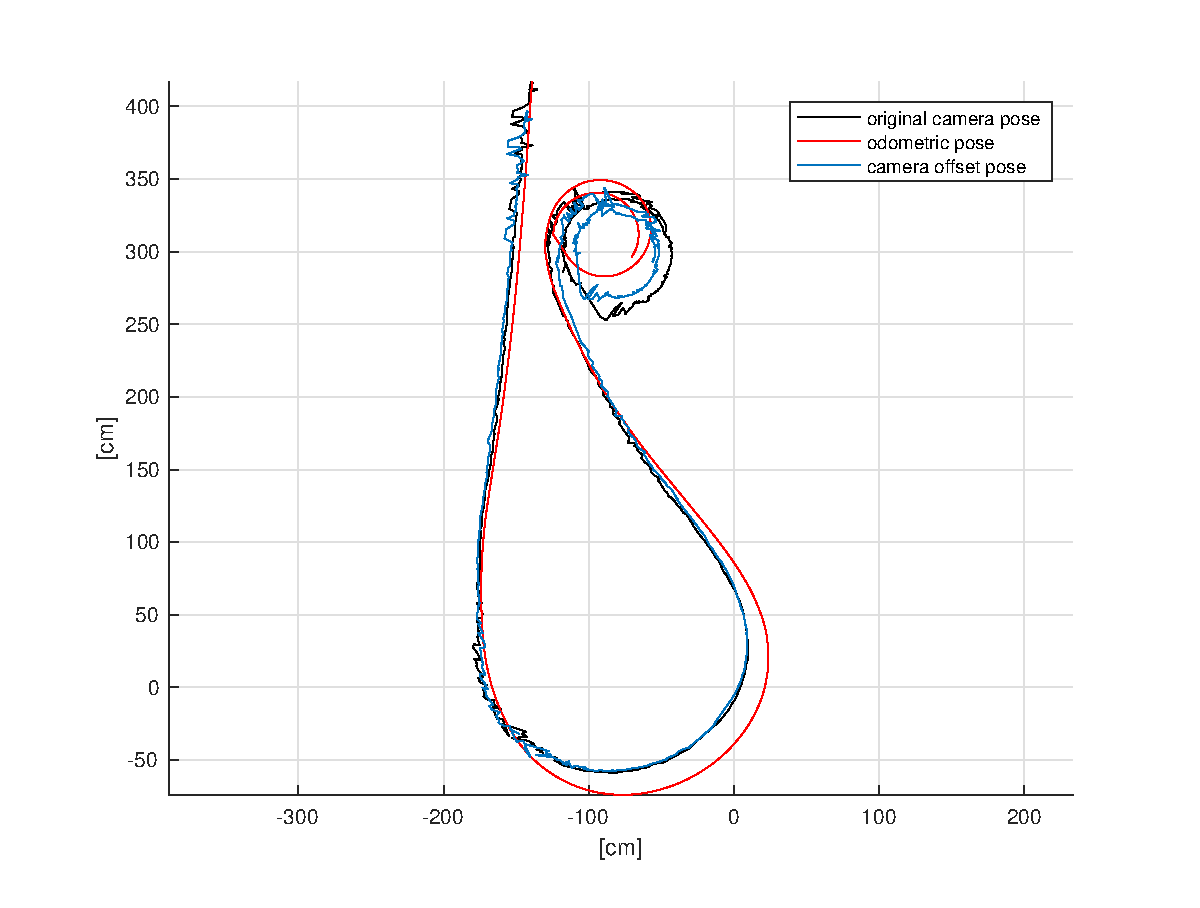
\includegraphics[width=0.45\textwidth]{recostropt_4}}
\caption{Optimal odometric and camera position, dataset: 4}
\label{fig:OptiOdo4}
\end{figure}